\chapter{Detalle del nodo de captura y detección}
\label{chap:anexo-captura}

\lettrine{E}{n} este anexo se detalla el procesamiento de imagen del nodo de captura, resumido en la sección~\ref{sec:nodo-camara}. El nodo se divide en dos componentes: el nodo de ROS~2, que gestiona la comunicación y los modos de funcionamiento, y un objeto que encapsula las operaciones de visión artificial con las que se obtiene el centroide de cada pegatina. Logrando desacoplar el procesamiento de imagen de la comunicación.

\section{Detección de las pegatinas por color}
\label{subsec:deteccion-etiquetas}

La detección hereda el procedimiento del trabajo de Mario López~\cite{tfgmario}. El fotograma se convierte al espacio HSV, que resiste mejor las variaciones de iluminación, y se genera una máscara binaria por pegatina con los píxeles que caen dentro del rango de su color. Están predefinidos para cada uno de los siete colores admitidos. Sobre cada máscara se encadenan una apertura morfológica, que elimina los píxeles aislados, y un cierre morfológico, que rellena los huecos de las regiones válidas.

Se extraen entonces los contornos externos y se toma el de mayor área, descartándolo si no supera un área mínima configurable. De este proceso se obtiene el rectángulo delimitador y el centroide de la pegatina, el significado para cada pegatina se describió en la sección~\ref{sec:arquitectura}. La figura~\ref{fig:deteccion-color} recorre estas etapas sobre un fotograma real.

\begin{figure}[tbp]
    \centering
    \begin{subfigure}[b]{0.48\textwidth}
        \centering
        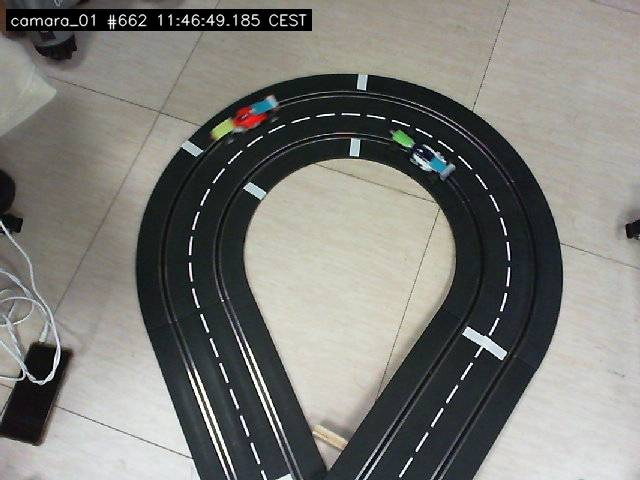
\includegraphics[width=\textwidth]{imaxes/IMPLEMENTACION/det_color_a_original.png}
        \caption{Fotograma capturado por la cámara}
        \label{fig:deteccion-color-a}
    \end{subfigure}
    \hfill
    \begin{subfigure}[b]{0.48\textwidth}
        \centering
        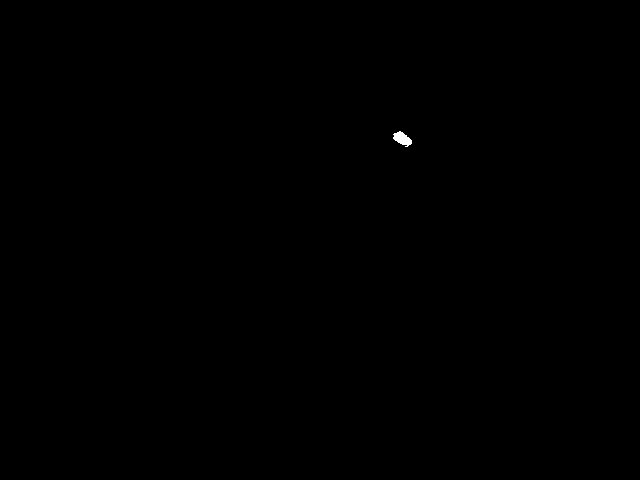
\includegraphics[width=\textwidth]{imaxes/IMPLEMENTACION/det_color_b_mascara.png}
        \caption{Máscara del color de la pegatina verde delantera del coche azul}
        \label{fig:deteccion-color-b}
    \end{subfigure}

    \vspace{0.7em}
    \begin{subfigure}[b]{0.34\textwidth}
        \centering
        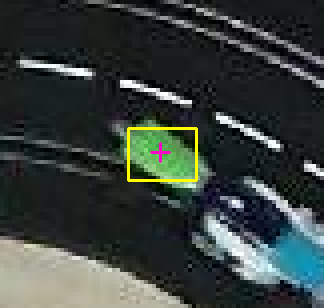
\includegraphics[width=\textwidth]{imaxes/IMPLEMENTACION/det_color_c_resultado.png}
        \caption{Rectángulo y centroide detectados después de realizar las operaciones pertinentes}
        \label{fig:deteccion-color-c}
    \end{subfigure}
    \caption{Ejemplo del proceso de detección que realiza el nodo camara para detectar una de las pegatinas del coche}
    \label{fig:deteccion-color}
\end{figure}

\section{Diferencias entre calibración y carrera}
\label{subsec:modos-funcionamiento}

El nodo implementa los dos modos descritos en la sección~\ref{sec:arquitectura}, y la diferencia entre ambos está en la región del fotograma sobre la que busca.

En calibración, cada detección de la pegatina delantera se añade a la lista que reconstruye la trayectoria del coche. Basta con la delantera, que es la que da una trayectoria limpia~\cite{tfgadrian}. Esto es porque la trasera puede quedar oculta a ratos y la ruta base debe registrarse sin interrupciones. Al mantener una trayectoria por coche, la cámara puede filtrar por carril en carrera y dos coches pueden compartir el color de la pegatina trasera. Durante todo este proceso se busca sobre el fotograma completo como el que se puede ver \ref{fig:deteccion-color-a}, es por ello que las pegatinas delanteras sí que tienen que ser de diferente color.

La calibración termina por coche, no para todo el sistema. El nodo se suscribe al \emph{topic} de calibración de cada coche configurado y, al recibir el aviso de que uno ha completado su vuelta, genera su máscara con los puntos acumulados. Desde ese momento la búsqueda de ese coche queda restringida a una franja alrededor del recorrido conocido, como recoge la figura~\ref{fig:mascara-trayectoria}.

\begin{figure}[tbp]
    \centering
    \begin{subfigure}[b]{0.32\textwidth}
        \centering
        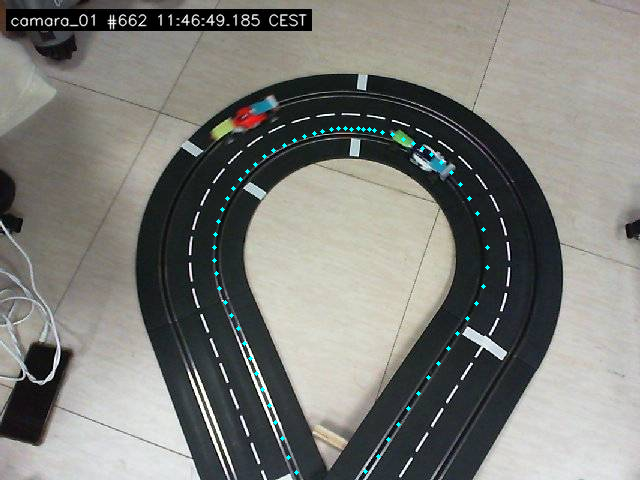
\includegraphics[width=\textwidth]{imaxes/IMPLEMENTACION/mascara_a_puntos.png}
        \caption{Posiciones acumuladas durante la vuelta de calibración}
        \label{fig:mascara-trayectoria-a}
    \end{subfigure}
    \hfill
    \begin{subfigure}[b]{0.32\textwidth}
        \centering
        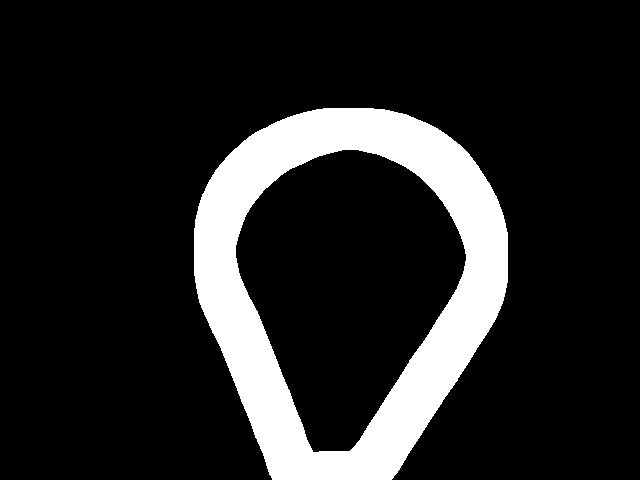
\includegraphics[width=\textwidth]{imaxes/IMPLEMENTACION/mascara_b_mascara.png}
        \caption{Máscara generada a partir de la posición que sigue el coche}
        \label{fig:mascara-trayectoria-b}
    \end{subfigure}
    \hfill
    \begin{subfigure}[b]{0.32\textwidth}
        \centering
        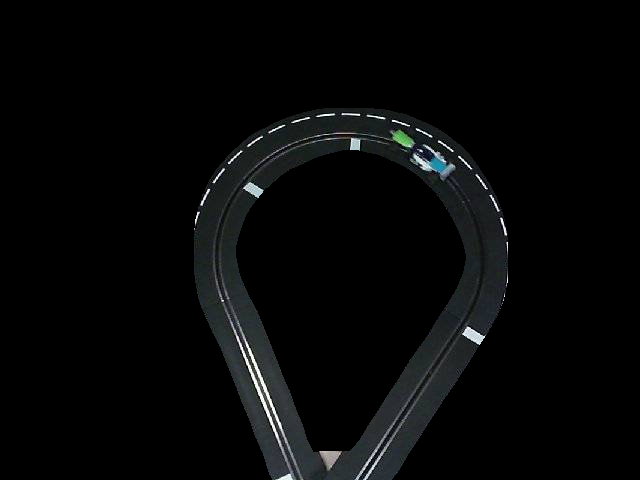
\includegraphics[width=\textwidth]{imaxes/IMPLEMENTACION/mascara_c_filtrado.png}
        \caption{Fotograma filtrado después de aplicar la mascara generada durante la calibración}
        \label{fig:mascara-trayectoria-c}
    \end{subfigure}
    \caption{Ejemplo de proceso de generación de la máscara de trayectoria para un coche. Deja fuera el carril contrario, con lo que el coche que circula por él deja de ser un falso positivo posible.}
    \label{fig:mascara-trayectoria}
\end{figure}

\section{Seguimiento mediante región de interés}
\label{subsec:seguimiento-roi}

En carrera la búsqueda se restringe a una región de interés de $150 \times 150$ píxeles centrada en la posición predicha para el coche. La predicción es la extrapolación lineal que introdujo Mario López~\cite{tfgmario}. Conocidas las dos últimas posiciones, el centro de la región es la actual más el vector de movimiento del último fotograma.

Sobre ella se aplica además la máscara de trayectoria, de modo que solo sobreviven los píxeles que pertenecen a la vez a la región y a las proximidades del carril; la intersección de ambos filtros procede también de los trabajos previos~\cite{tfgmario,tfgadrian}. La detección de las pegatinas (\ref{subsec:deteccion-etiquetas}) se realiza sobre esa imagen reducida, se puede ver un ejemplo en \ref{fig:roi-filtrado}. El problema que presenta hacerlo de esta manera es que sus coordenadas son relativas a la región y hay que trasladarlas al sistema de referencia de la cámara antes de publicarlas.

\begin{figure}[tbp]
    \centering
    \begin{subfigure}[b]{0.55\textwidth}
        \centering
        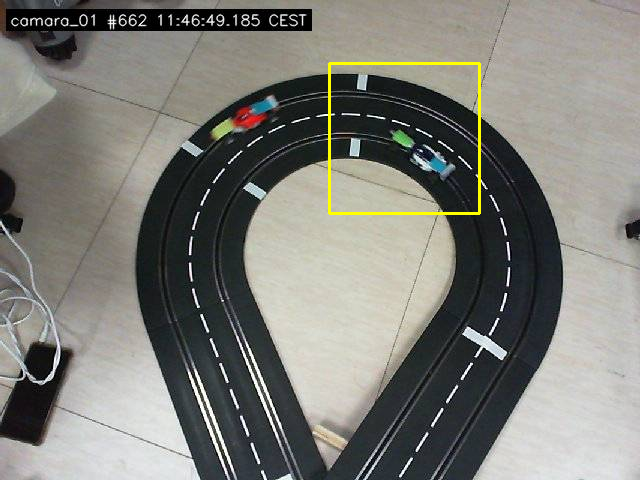
\includegraphics[width=\textwidth]{imaxes/IMPLEMENTACION/roi_a_recuadro.png}
        \caption{Región de interés marcada sobre todo el fotograma}
        \label{fig:roi-filtrado-a}
    \end{subfigure}
    \hfill
    \begin{subfigure}[b]{0.38\textwidth}
        \centering
        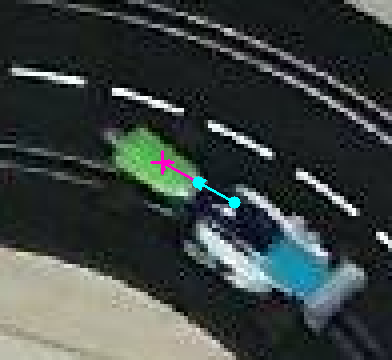
\includegraphics[width=\textwidth]{imaxes/IMPLEMENTACION/roi_b_extrapolacion.png}
        \caption{Extrapolación de la posición}
        \label{fig:roi-filtrado-b}
    \end{subfigure}

    \vspace{0.7em}
    \begin{subfigure}[b]{0.32\textwidth}
        \centering
        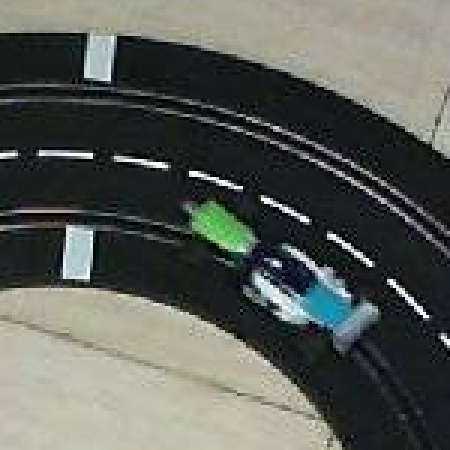
\includegraphics[width=\textwidth]{imaxes/IMPLEMENTACION/roi_c_recorte.png}
        \caption{Recorte de la región}
        \label{fig:roi-filtrado-c}
    \end{subfigure}
    \hspace{0.04\textwidth}
    \begin{subfigure}[b]{0.32\textwidth}
        \centering
        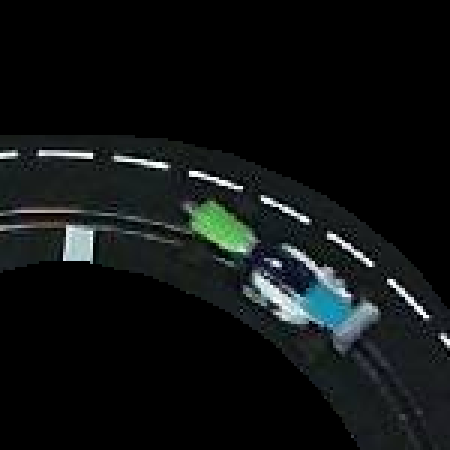
\includegraphics[width=\textwidth]{imaxes/IMPLEMENTACION/roi_d_filtrado.png}
        \caption{Región tras la intersección entre la mascara y el ROI}
        \label{fig:roi-filtrado-d}
    \end{subfigure}
    \caption{Explicación del proceso de obtención del ROI y aplicación dentro del sistema. En el detalle, las dos flechas encadenadas son el desplazamiento medido entre los dos últimos fotogramas. La cruz marca la posición predicha, que en este fotograma cae a 1,6 píxeles de la real. El último panel es lo único que llega al detector de color.}
    \label{fig:roi-filtrado}
\end{figure}

\section{Readquisición del seguimiento}
\label{subsec:readquisicion}

Las oclusiones son habituales en un circuito de Scalextric~\cite{tfgmario}, y un derrape brusco puede alejar el coche de la posición predicha. En ambos casos la detección fracasa y hay que recuperar el seguimiento.

La estrategia es ampliar progresivamente la zona de búsqueda. Cada fotograma sin detección incrementa el tamaño de la región en 50 píxeles, hasta abarcar como máximo la imagen completa. Los trabajos previos pasaban de golpe a examinar toda la proximidad de la trayectoria; el crecimiento gradual acota el coste de los fotogramas inmediatamente posteriores a la pérdida.

Al perder el seguimiento se descartan las posiciones anteriores, como ya hacía Mario López~\cite{tfgmario}, para que la extrapolación no combine un punto previo a la pérdida con el primero posterior y sitúe la región lejos del coche. La primera detección tras readquirir centra la región sobre la posición encontrada.

\section{Detección de la línea de meta}
\label{subsec:deteccion-meta}

La línea de meta se señaliza con una etiqueta alargada de un color reservado que atraviesa la pista. Se detecta una sola vez, al arrancar el nodo, porque su posición no cambia durante la carrera.

El procedimiento empleado para la detección de la línea de meta es el de Adrián Rego~\cite{tfgadrian}. Al igual que en la detección de las pegatinas, el fotograma se convierte al espacio de color HSV y se genera una máscara binaria con el rango del color reservado para la meta (se puede cambiar desde el fichero de configuración \ref{subsec:params-yaml}), de forma que se genera una mascara binaria con los píxeles de la etiqueta. Sobre está se aplica un cierre morfólogico con un tamaño de \emph{kernel} muy grande, porque los raíles y las ranuras de la pista atraviesan la etiqueta y la fragmentan en trozos que hay que unir en una única región. Sobre está región se calcula el rectángulo de área mínima que lo encierra, el cual, a diferencia del rectángulo delimitador convencional, puede estar rotado y se adapta así a la orientación real de la linea de meta. De sus cuatro vértices se identifican los dos lados cortos comparando las longitudes de las aristas adyacentes, y el segmento que une sus puntos medios define la línea de meta. La figura~\ref{fig:deteccion-meta} muestra las tres etapas del proceso.

\begin{figure}[tbp]
    \centering
    \begin{subfigure}[b]{0.32\textwidth}
        \centering
        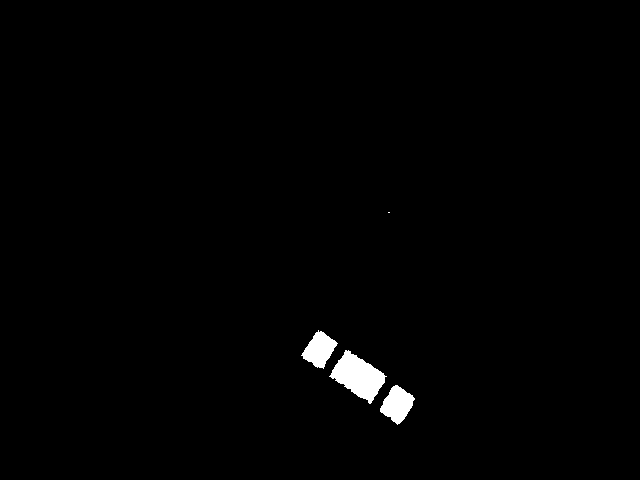
\includegraphics[width=\textwidth]{imaxes/IMPLEMENTACION/meta_a_mascara.png}
        \caption{Máscara del color de la meta}
        \label{fig:deteccion-meta-a}
    \end{subfigure}
    \hfill
    \begin{subfigure}[b]{0.32\textwidth}
        \centering
        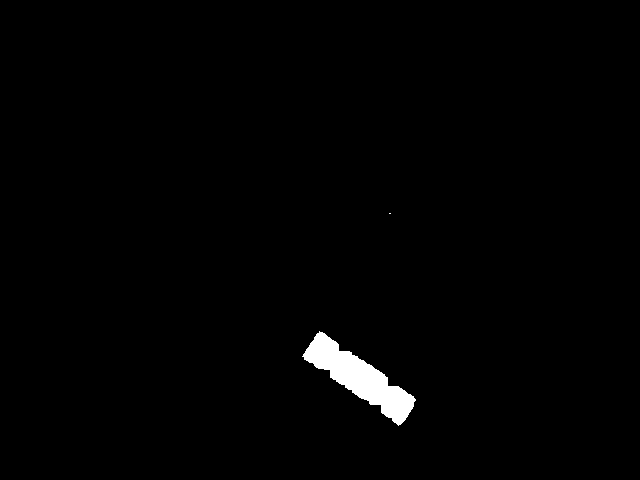
\includegraphics[width=\textwidth]{imaxes/IMPLEMENTACION/meta_b_cierre.png}
        \caption{Tras el cierre morfológico}
        \label{fig:deteccion-meta-b}
    \end{subfigure}
    \hfill
    \begin{subfigure}[b]{0.32\textwidth}
        \centering
        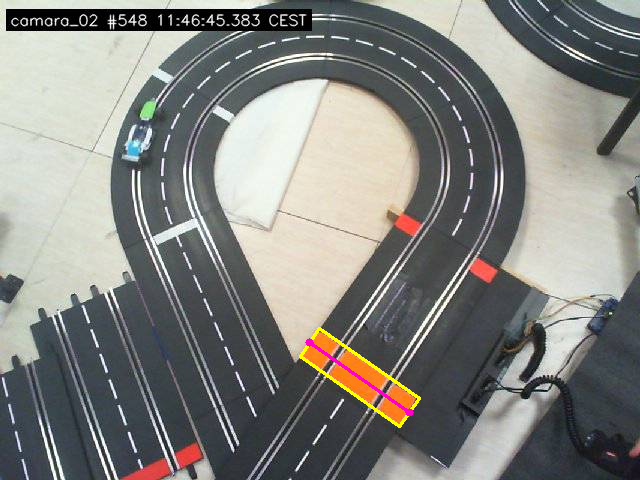
\includegraphics[width=\textwidth]{imaxes/IMPLEMENTACION/meta_c_segmento.png}
        \caption{Rectángulo y segmento}
        \label{fig:deteccion-meta-c}
    \end{subfigure}
    \caption{Detección de la línea de meta en la cámara~2. Los raíles parten la etiqueta en tres trozos que el cierre morfológico vuelve a unir; sobre la región resultante se ajusta el rectángulo de área mínima, rotado, y los puntos medios de sus lados cortos dan el segmento de meta.}
    \label{fig:deteccion-meta}
\end{figure}

Cada nodo la busca al arrancar y, si no la ve, no publica línea de meta alguna. Por lo que en un despliegue multicámara solo lo hace la que observa la linea y generando el mensaje correspondiente (tabla~\ref{tab:mensajes}). No hay, por tanto, una cámara de meta designada de antemano por el usuario.
